\newpage

\hoffset=0pt

\newgeometry{left=7.5cm,right=2cm, marginparsep=15pt, marginparwidth=4.2cm,top=2cm}


\cxset{style16/.style={
 chapter opening=any,
 name={},
 numbering=arabic,
 number color= thegray,
 number font-size=\HHUGE,
 number font-family=\rmfamily,
 number font-weight=\bfseries,
 number before=\leftskip-4cm\vbox to 0cm\bgroup\vspace*{5cm},
 number after=\egroup\vskip0pt\par,
 number dot=,
 number position=leftname,
 chapter font-family=\sffamily,
 chapter font-weight=\normalfont,
 chapter font-size=\Large,
 chapter before={},
 chapter after={\begin{picture}(0,0)
                          \put(-50pt,\dimexpr-\textheight+\footskip+20pt\relax){\parbox{\marginparwidth}{\textbf{Napoleon}\par\lorem}}%
                        \end{picture}},
 chapter color={black!90},
 title beforeskip={\par\hspace*{4cm}\thinrule\vskip0pt\hspace*{4cm}\vbox\bgroup},
 title afterskip={\vspace*{50pt}\par\egroup},
 title before={},
 title after=,
 title font-color= black!80,
 title font-weight=\normalfont,
 title font-family=\rmfamily,
 title font-shape=\upshape,
 title font-size=\HUGE,
 chapter title width=\textwidth,
 chapter title align=raggedright,
 header style=empty,
 subsection numbering=none,
 subsection color=teal,
 subsection align=teal,
 header style=empty,
 }}

\renewsubsection


\def\fullpageimage{%
       \leavevmode\mbox{}
       \vbox{%
        \parindent0pt
       \vfill
       \fbox{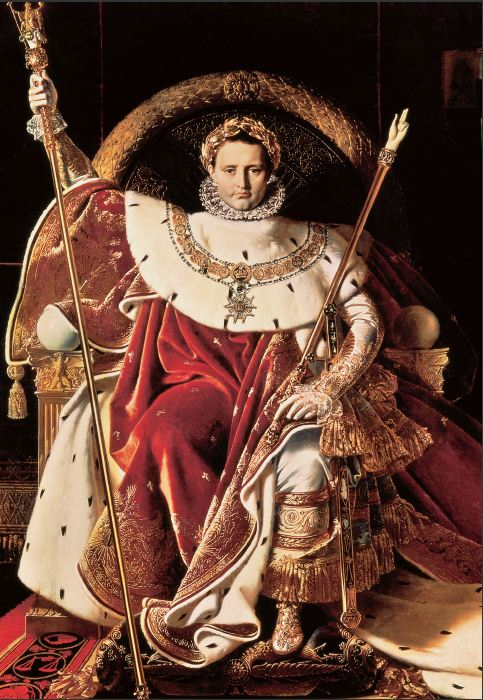
\includegraphics[height=\pdfpageheight]{./images/napoleon.jpg}}%
       }%
}


\cleardoublepage

\fullpageimage

\cxset{style16}
\chapter{Victorian England:\\ Introduction 16}
\label{style16}
This design from a Social Sciences book had to be set into two vboxes and negative skips allowed to line
up the numbers. Once I am totally happy with it, I will add parameter adjustments, as well as a bit of automation of length calculations.
\thispagestyle{empty}

\medskip

\begin{figure}[ht]
\centering
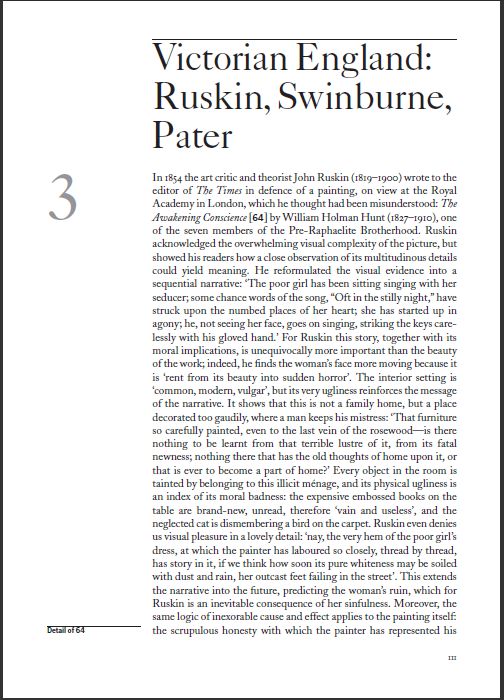
\includegraphics[width=0.35\textwidth]{./chapters/chapter16.png}
\end{figure}
\lipsum[2]

\cxset{geometry marginparsep/.code=\setlength\marginparsep{#1},
          geometry marginparwidth/.code=\setlength{\marginparwidth}{#1}}

\section{Technical notes}

This design looks simple but takes a bit of effort to achieve it, especially due to the tendency of LaTeX and the TeX engine to make decisions for you. Firstly we cannot reset the page geometry between the image and the chapter, as this will either result in unpredictable behaviour or if you use the \cs{newgeometry} macro, it will for certain leave a blank page in between.

\begin{description}
\item [image sizing] The image is set at \textbf{width=paperwidth}. This can vary depending on the page geometry and the image aspect ratio. In general you may need to ensure that your image has the same aspect ratio as the page to avoid problems with placement and the generation of extra blank pages.
\item [image caption] The image caption is placed using the picture environment, so that it can be typeset absolutely, feel free to use TikZ for the same purpose. We also use Heiko Oberdiek's the \pkg{picture} package to make calculations easier by specifying actual dimensions and not needing to strip the point.
\end{description}



\restoregeometry

